\subsection{Aligned event counters}\label{app:event-counters}

\Cref{fig:event-counters} aligns two committed histories sharing logged round
identifiers. The consecutive insertion records bracket the full admission
window; rounds without a recorded insertion are retained as zero counts. An insertion does not imply an adapter admission.

\begin{figure}[tb]
  \centering
  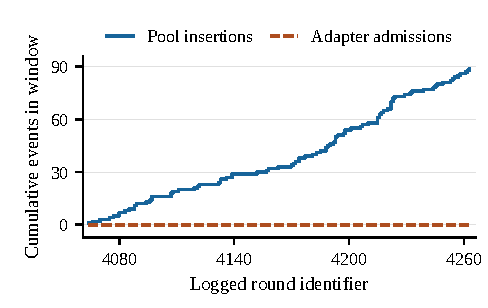
\includegraphics[width=\linewidth]{figures/fig_event_counters.pdf}
  \caption{\textbf{Pool insertions accumulate without adapter admission.}
  All 200 admission decisions in rounds 4064--4263, aligned with every
  program/context insertion in the committed history over those round
  identifiers. Blue: cumulative pool insertions; orange: cumulative adapter
  admissions. The window contains 89 insertions and zero adapter
  admissions. Each count starts at the window boundary and includes all
  events through the displayed round. These are distinct engineering-event
  counts, not independent proposal outcomes or evidence of learning gain.
  Scope: \cref{sec:method-status}.}
  \label{fig:event-counters}
\end{figure}
